\section{Classification algorithms} %TODO: Vukans corrections!

In general, classification algorithms are a type of supervised machine learning algorithms.
In machine learning, the parameters $\theta$ of a function $f$, also called a model, are optimized, so that predictions $\hat{y}=f(x|\theta)$ can be made that solves a given problem based on some input $x$.
Supervised machine learning is the optimization, also called training, of such models based on a dataset that contains the desired target $y$ for a given input. 
In classification algorithms, $y$ is a categorical variable and $\hat{y}$ can contain either discrete values or estimated probabilities. 
Therefore, classification algorithms try to assign a class to something (sample) based on measured quantities (features) that represent it. %TODO: "something" different word
For example, the main algorithm of this thesis evaluates the measured data of a $pp$-collision to estimate the class of the $B$ meson produced in this event.
The classification algorithms used in this thesis are described in the following sections.

\subsection{Boosted Decision Tree (BDT)}
\label{sec:BDT}

A Boosted Decision Tree (BDT) is an ensemble of multiple different decision trees trained and evaluated on the principles of gradient boosting.
Decision trees are binary trees with a decision condition at each node and a prediction score for each leaf.
The decisions are made on a single feature at each node.
The weighted sum of the prediction scores of all trees is then transformed using the logistic function to resemble a probability that the given sample belongs to one of the classes.
In gradient boosting the decision trees are trained iteratively, so that at each step the weighted sum of all previous decision trees and the current decision tree minimizes a given objective function.
To find the minimum, the gradient of the objective function with respect to the model parameters is calculated.
%All BDTs in this thesis are implemented in Python using the library XGBoost \cite{xgboost}.

\subsection{Neural Network (NN)}
\label{sec:NN}

\begin{figure}
    \centering
    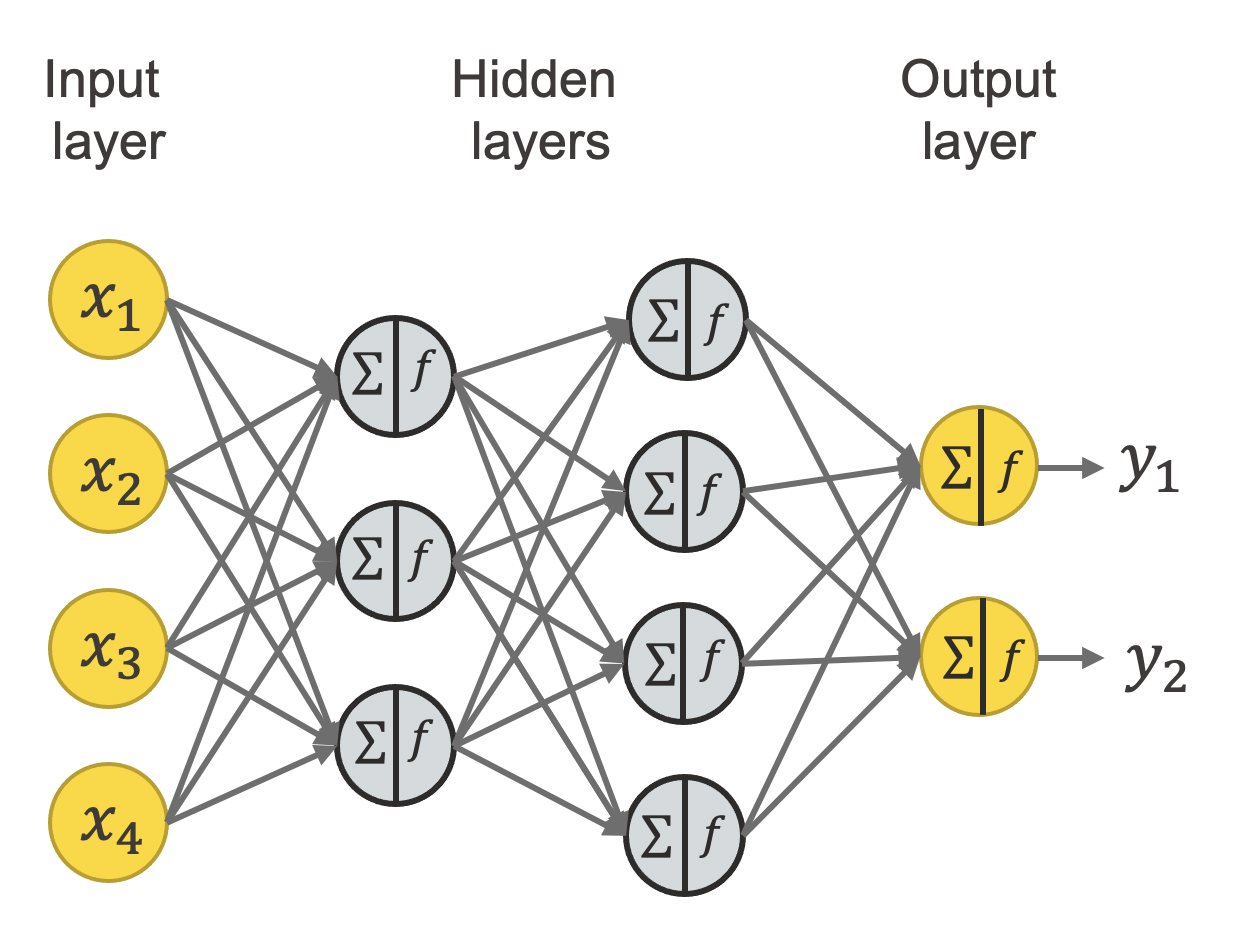
\includegraphics[width=0.5\textwidth]{images/NN_schematic.png}
    \caption{Example of a fully connected, feedforward neural network \cite{NN_schematic}.}
    \label{fig:NN_schematic}
\end{figure}

A Neural Network (NN) consists of multiple layers of (artificial) neurons to calculate an output vector $\hat{y}$ based on an input vector $x$.
The amount of layers and the amount of neurons per layer can be arbitrarily chosen based on the complexity of the problem.
\autoref{fig:NN_schematic} shows an example NN with 4 layers and is the basis of the following explanation.
Here, neurons are visualized as circles and represent a scalar number called activation $a$. 
The inputs of a neuron are marked by arrows from left to right and each arrow also represents a weight $w$.
The activation of each neuron is calculated by feeding the weighted sum 
\begin{equation*}
    z = \sum_{i \in \{\text{input neurons}\}} w_i \cdot a_i + b \, 
\end{equation*}
into a function $f(z)$ called the activation function.
$b$ is called the bias-weight of a neuron.
The activation functions used in this thesis are 
\begin{align*}
    f_\text{ReLU}(z) &= \max(0, z) \:\:\text{  and} \\
    f_\text{Sigmoid}(z) &= \frac{1}{1+e^{-z}} \, .
\end{align*}
The activations of the first layer are the values of $x$, and the activations of the last layer are used as the values of $\hat{y}$.
The layers in between the first and the last layer are called hidden layers.

To produce the desired outputs, the weights of a NN have to be adjusted in an iterative training process.
During the training process it is tried to find the minimum of a loss function that describes how well the NN solves the given problem based on the given target $y$.
Before the first iteration, all weights are initialized at random.
Each iteration then calculates the NN outputs and estimates the gradient of the loss function with respect to the weights.
Based on the gradient, the weights are adjusted towards the estimated minimum.
The step size at each iteration is determined by an optimizer algorithm.
This thesis uses the loss function binary cross entropy in combination with the optimizer Adam.
% TODO: bce formula and reference for Adam

NNs are prone to describe the training data too well, so that the model does not perform well on unseen data.
To prevent this overtraining, the regularization techniques used in this thesis are early stopping and dropout.

Early stopping calculates the loss on a validation dataset that is not used to adjust the weights.
If the loss does not improve for $N$ iterations the training is stopped and the weights of the best iteration based on this validation loss are used in the fitted NN.
This way, further adjusting of the NN to the training data is prevented and only the best results on the validation data are used.

In dropout, at each training iteration a random subset of neurons are disabled and only the remaining NN is evaluated and optimized.
Essentially, at each training iteration a smaller NN is trained and the co-dependence of neurons is reduced.
This makes the NN more robust and reduces overtraining.

\subsection{DeepSet}
\label{sec:DeepSet}

A DeepSet is an extension of NNs to allow inputs of sets of vectors.
DeepSets can therefore be used to solve problems where the data of each sample contains a variable length list and where the solution should be invariant under permutations of this list.
In this thesis, a DeepSet is used to classify $pp$-collision events that contain different amounts of tracks of which the order in the data should not matter.

The basic idea of DeepSets is that a function is invariant under permutations of the instances $x$ in a set $X$ if it can be written in the form 
\begin{equation*}
    f(X) = \rho \left( \sum_{x \in X} \phi (x) \right) \, .
\end{equation*}
This is also true, if the sum is replaced with any permutation invariant function.
In DeepSets $\rho$ and $\phi$ are represented by NNs and can be vector-valued \cite{deepset}.
In other words, a $\phi$-network first extracts some features about each instance in the set.
The feature values of all instances are then summed up and fed into a $\rho$-network that calculates the desired output.

The training of a DeepSet is fully analogous to the training of a NN.
The only difference is that a DeepSet consists of two NNs that are trained together.
%All DeepSets used in this thesis are implemented in Python using the library Pytorch \cite{pytorch}.




% A NN consists of multiple layers of (artificial) neurons to calculate an output vector $\hat{y}$ based on an input vector $x$.
% The amount of layers and the amount of neurons per layer can be arbitrarily chosen based on the complexity of the problem.
% A neuron represents a scalar number called activation that is calculated based on the weighted connections to the neurons of the previous % layer.
% The first layer of neurons is called the input layer and its activations are the values of $x$.


% A NN consists of multiple layers of (artificial) neurons to calculate an output vector $\hat{y}$ based on an input vector $x$.
% The amount of layers and the amount of neurons per layer can be arbitrarily chosen based on the complexity of the problem.
% A neuron calculates a scalar number called activation based on the activations of all neurons from the previous layer.
% The first layer of neurons is called the input layer and its activations are the values of $x$.
% When $a$ represents the activations of the previous layer, the linear activation of a single neuron in the next layer is
% \begin{equation*}
%     z = \sum_i w_i \cdot a_i + b \, .
% \end{equation*}
% $w_i$ is the weight associated with the connection to 
% 
% The activation of each other neuron is calculated through an activation function $f(z)$, where 
% \begin{equation*}
%     z = \sum_i w_i \cdot a_i + b \, .
% \end{equation*}
% $w_i$ is the weight of a connection between two neurons
% , the last layer is called the output layer and all layers in between are called hidden layers.
% 
% \autoref{fig:NN_schematic} shows an example NN with 4 layers.
% Each neuron is represented as a circle and the arrows represent the weighted connections between two neurons.
% 
% 
% A NN passes an input vector $x$ through multiple layers of (artificial) neurons to calculate an output vector $\hat{y}$ that may have a % different length than $x$.
% The amount of layers and the amount of neurons per layer can be arbitrarily chosen based on the complexity of the problem.
% A schematic of a NN with 3 layers is shown in \autoref{fig:NN_schematic}.
% Here, each neuron is represented by a circle and the arrows
% A neuron with an input vector $a$ first calculates a scalar 
% \begin{equation*}
%     z = \sum_i w_i \cdot a_i + b
% \end{equation*}
% called linear activation. 
% The vector $w$ and the scalar $b$ contain weights, that have to be optimized in the training process.
% Usually, this linear activation is then further transformed using an activation function.
% The activation functions used in this thesis are 
% \begin{align*}
%     \text{ReLU}(z) &= \max(0, z) & and \\
%     \text{Sigmoid}(z) &= \frac{1}{1+e^{-z}} \, .
% \end{align*}

